\subsection{DAC Power Amp} \label{subsec:DAC_Filter}
The system is to test impedance over a broad range of \SIQ{100}{\milli\ohm} to \SIQ{100}{\mega\ohm}, according to requirement §3 from section \ref{ch:SystemRequirements}. In order to excite impedances, especially in the range of \SIQ{10}{\ohm} and lower, a power amplifier is required. This amplifier must be capable of driving both reactive and passive devices. This is achieved by the use of controlled output impedance and the utilized range resistors used to measure the DUT current. 

The amplifier is designed as a class AB amplifier output stage and a high speed op-amp. The circuit used can be seen in figure \ref{fig_7_1_1_5_DAC_POWER_AMP}.

\begin{figure}[H]
    \centering
    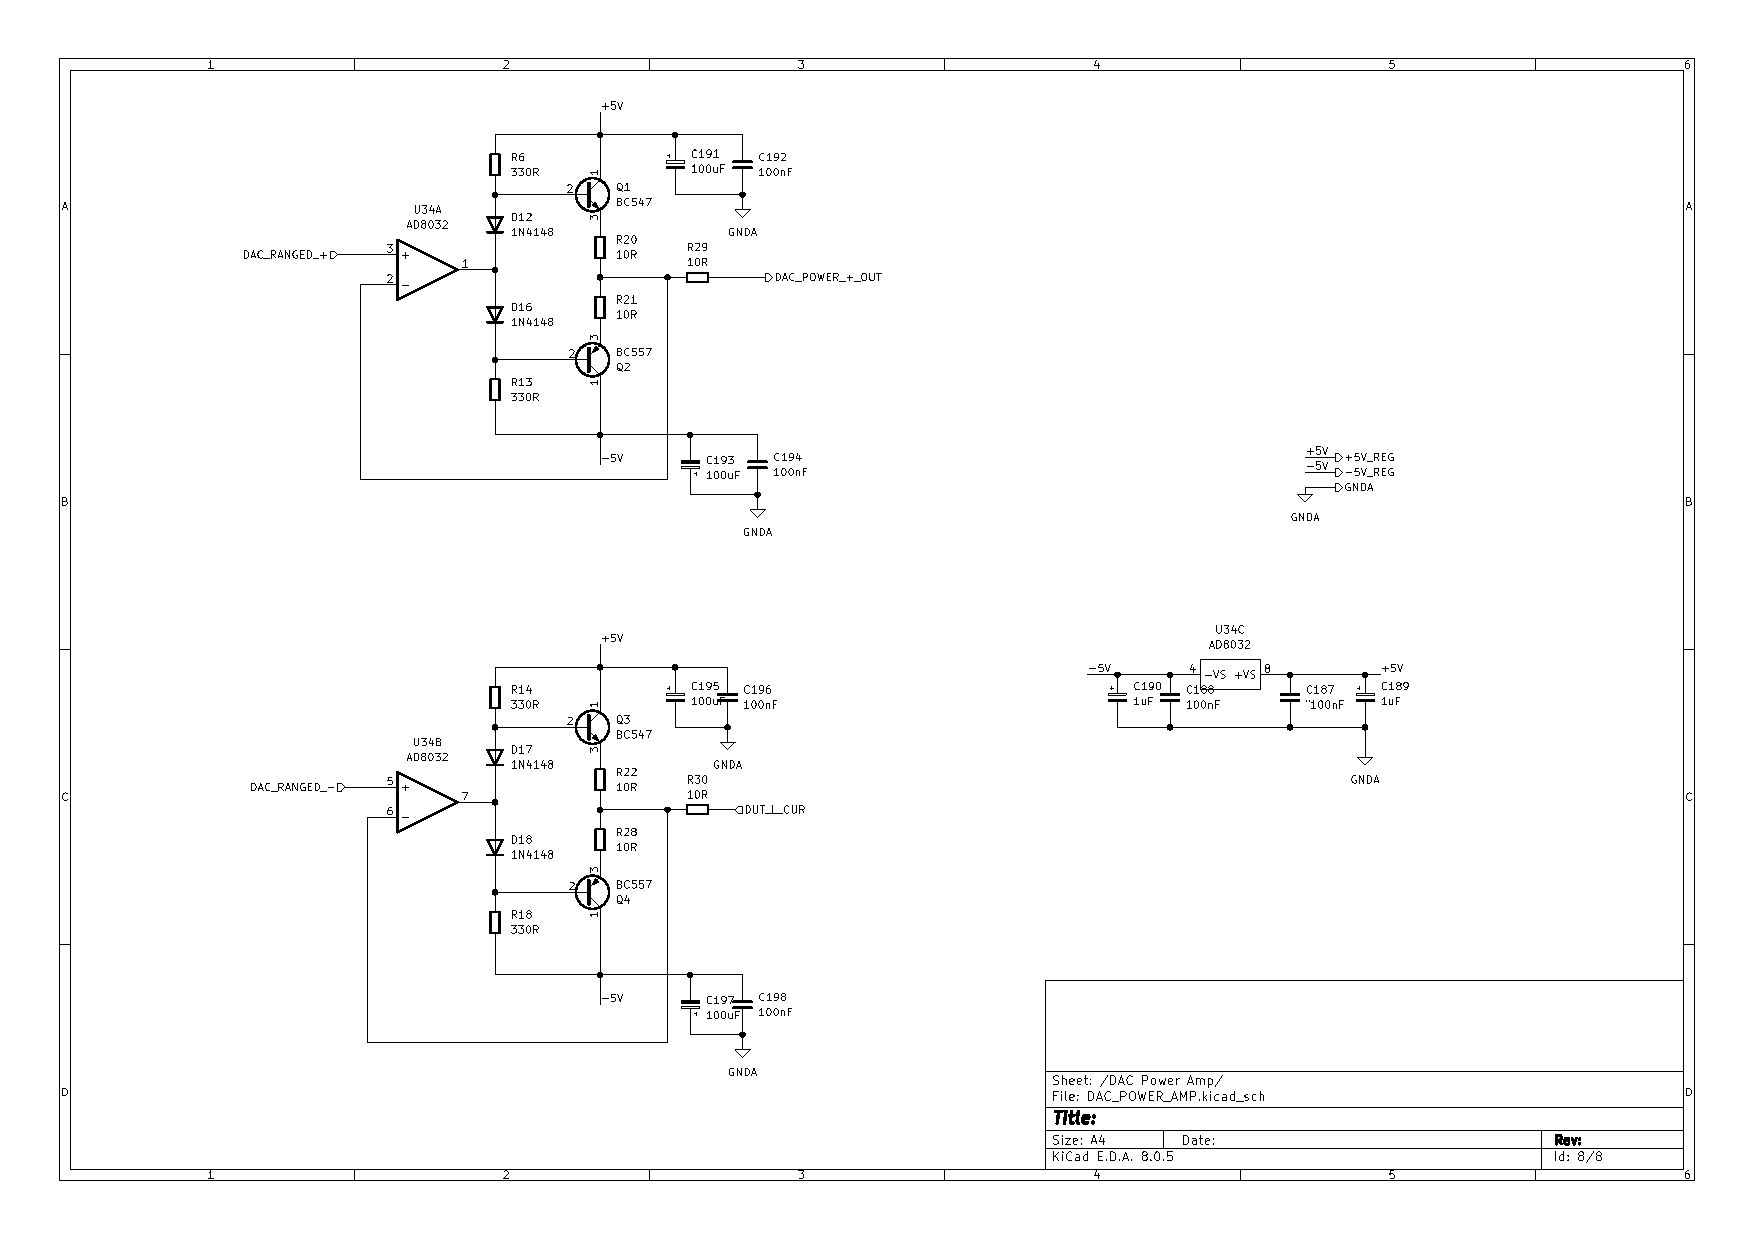
\includegraphics[clip, trim=150 320 415 40, width=0.9\textwidth]{Sections/7_SystemDesign/Figures/7_1_1_5_DAC Power Amp.pdf}
    \caption{DAC power amplifier circuit, positive side of the differential output.}
    \label{fig_7_1_1_5_DAC_POWER_AMP}
\end{figure}

About \SIQ{15}{\milli\ampere} of bias current for the output stage has been chosen. From BC547B and BC557 datasheets, \cite{BC547_datasheet} \cite{BC557_datasheet}, the base-emitter voltage can be found to be roughly \SIQ{730}{\milli\volt} at a collector current of \SIQ{15}{\milli\ampere}. This bias-current is set by the use of a simply diode. This adds some thermal stability, given they are thermally closely linked, as the temperature coefficient of a diode is negative, whilst positive for a transistor. The required DC current for a 1n4148 diode to have a voltage-drop of \SIQ{730}{\milli\volt} is estimated to \SIQ{12}{\mA}. The supply voltage is from a split supply of $\pm$ \SIQ{5}{\volt}, resulting in a total supply voltage of \SIQ{10}{\volt}. Assuming that the two biasing diodes, D12 and D16 in figure \ref{fig_7_1_1_5_DAC_POWER_AMP}, are matched the voltage across the biasing resistors R6 and R13 will be $10-2\cdot0.73 = $\SIQ{8.54}{\volt}. Combined series resistance of R6 and R13 can be estimated as $\frac{8.54 V}{0.012 A} = $ \SIQ{712}{\ohm}. Resistors of \SIQ{330}{\ohm} has been chosen, producing a biasing current of \SIQ{12.9}{\milli\ampere}.

To increase the input impedance and reduce output distortion of the amplifier, an op-amp is used with the output class AB stage in its feedback loop. The used op-amp is an \SIQ{80}{\mega\hertz} GBW op-amp, AD8032 \cite{AD8032_datasheet}. 

\subsubsection{Stability}
Driving reactive, especially capacitive loads can pose a challenge to any feedback system with a phase margin less than \SIQ{90}{\degree}. The typical phase-margin of an op-amp is in the range of \SIQ{45}{\degree}, leading to potential instability when driving capacitive loads.

A way to counteract the risk of instability, is to introduce a zero in the transfer function of the feedback path by inserting a series resistance with the output of the feedback system, this is also known as an isolation resistor. This resistor should be placed outside of the feedback loop, the value of this resistor will depend upon the load capacitor. This indicates that a stability analysis of the DAC power amp should be conducted, as it is very likely that a user would load the system with a capacitive load. This analysis is based on the block diagram of the differential DAC output, depicted as a block diagram in figure \ref{fig_7_1_1_5_DAC_POWER_AMP_BLOCK}. 


\begin{figure}[H]
    \centering
    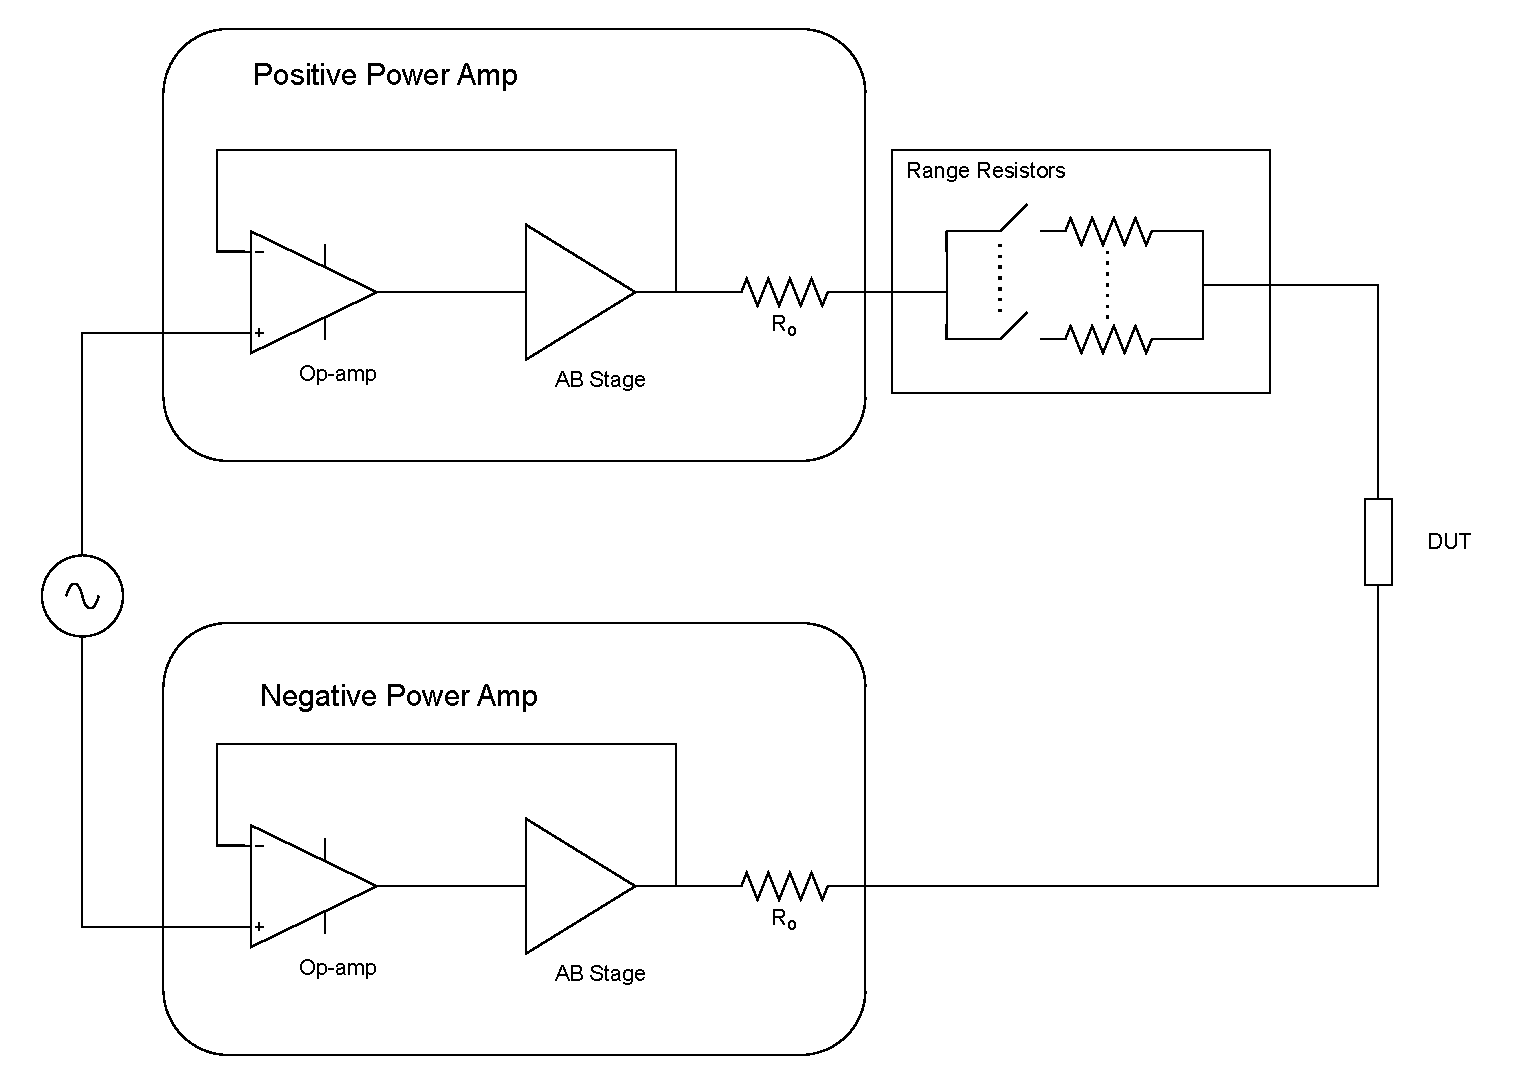
\includegraphics[clip, trim=0 0 0 0, width=0.9\textwidth]{Sections/7_SystemDesign/Figures/DAC_POWER_BLOCK.pdf}
    \caption{Block diagram of the differential DAC power amp output stage.}
    \label{fig_7_1_1_5_DAC_POWER_AMP_BLOCK}
\end{figure}

The stability analysis is simplified by only looking at the positive side of the differential output seen in figure \ref{fig_7_1_1_5_DAC_POWER_AMP_BLOCK}. Here $R_o$ is then replaced by $2\cdot R_o$. One thing to take note of here, is that the range resistors can be used both as current shunts and isolation resistors. The stability analysis aims to ensure that when the output is capacitively loaded, the appropriate range resistor will establish stability.

To analyze the output stage, the op-amp is modelled as a two pole \SIQ{80}{\mega\hertz} GBW, \SIQ{30}{\degree} phase margin op-amp with \SIQ{80}{\decibel} open-loop DC gain, based on the datasheet information of the used AD8032 \cite{AD8032_datasheet}. The class AB output stage is modelled as a small signal emitter follower. Using a small signal model might seem somewhat unsuitable for the output stage, as it does not operate with small signals. The small signal model has however proved to produce approximately accurate bandwidth information, even for large signals.

The small signal model for the 

\begin{figure}[H]
    \centering
    \includegraphics[clip, trim=50 20 100 100, width=0.9\textwidth]{Sections/7_SystemDesign/Figures/DAC_POWER_ss.pdf}
    \caption{Small signal model of the differential output power stage.}
    \label{fig_7_1_1_5_DAC_POWER_AMP_ss}
\end{figure}